% Options for packages loaded elsewhere
\PassOptionsToPackage{unicode}{hyperref}
\PassOptionsToPackage{hyphens}{url}
\PassOptionsToPackage{dvipsnames,svgnames,x11names}{xcolor}
%
\documentclass[
  letterpaper,
  DIV=11,
  numbers=noendperiod]{scrartcl}

\usepackage{amsmath,amssymb}
\usepackage{lmodern}
\usepackage{iftex}
\ifPDFTeX
  \usepackage[T1]{fontenc}
  \usepackage[utf8]{inputenc}
  \usepackage{textcomp} % provide euro and other symbols
\else % if luatex or xetex
  \usepackage{unicode-math}
  \defaultfontfeatures{Scale=MatchLowercase}
  \defaultfontfeatures[\rmfamily]{Ligatures=TeX,Scale=1}
\fi
% Use upquote if available, for straight quotes in verbatim environments
\IfFileExists{upquote.sty}{\usepackage{upquote}}{}
\IfFileExists{microtype.sty}{% use microtype if available
  \usepackage[]{microtype}
  \UseMicrotypeSet[protrusion]{basicmath} % disable protrusion for tt fonts
}{}
\makeatletter
\@ifundefined{KOMAClassName}{% if non-KOMA class
  \IfFileExists{parskip.sty}{%
    \usepackage{parskip}
  }{% else
    \setlength{\parindent}{0pt}
    \setlength{\parskip}{6pt plus 2pt minus 1pt}}
}{% if KOMA class
  \KOMAoptions{parskip=half}}
\makeatother
\usepackage{xcolor}
\usepackage[top=30mm,left = 30mm]{geometry}
\setlength{\emergencystretch}{3em} % prevent overfull lines
\setcounter{secnumdepth}{5}
% Make \paragraph and \subparagraph free-standing
\ifx\paragraph\undefined\else
  \let\oldparagraph\paragraph
  \renewcommand{\paragraph}[1]{\oldparagraph{#1}\mbox{}}
\fi
\ifx\subparagraph\undefined\else
  \let\oldsubparagraph\subparagraph
  \renewcommand{\subparagraph}[1]{\oldsubparagraph{#1}\mbox{}}
\fi

\usepackage{color}
\usepackage{fancyvrb}
\newcommand{\VerbBar}{|}
\newcommand{\VERB}{\Verb[commandchars=\\\{\}]}
\DefineVerbatimEnvironment{Highlighting}{Verbatim}{commandchars=\\\{\}}
% Add ',fontsize=\small' for more characters per line
\usepackage{framed}
\definecolor{shadecolor}{RGB}{241,243,245}
\newenvironment{Shaded}{\begin{snugshade}}{\end{snugshade}}
\newcommand{\AlertTok}[1]{\textcolor[rgb]{0.68,0.00,0.00}{#1}}
\newcommand{\AnnotationTok}[1]{\textcolor[rgb]{0.37,0.37,0.37}{#1}}
\newcommand{\AttributeTok}[1]{\textcolor[rgb]{0.40,0.45,0.13}{#1}}
\newcommand{\BaseNTok}[1]{\textcolor[rgb]{0.68,0.00,0.00}{#1}}
\newcommand{\BuiltInTok}[1]{\textcolor[rgb]{0.00,0.23,0.31}{#1}}
\newcommand{\CharTok}[1]{\textcolor[rgb]{0.13,0.47,0.30}{#1}}
\newcommand{\CommentTok}[1]{\textcolor[rgb]{0.37,0.37,0.37}{#1}}
\newcommand{\CommentVarTok}[1]{\textcolor[rgb]{0.37,0.37,0.37}{\textit{#1}}}
\newcommand{\ConstantTok}[1]{\textcolor[rgb]{0.56,0.35,0.01}{#1}}
\newcommand{\ControlFlowTok}[1]{\textcolor[rgb]{0.00,0.23,0.31}{#1}}
\newcommand{\DataTypeTok}[1]{\textcolor[rgb]{0.68,0.00,0.00}{#1}}
\newcommand{\DecValTok}[1]{\textcolor[rgb]{0.68,0.00,0.00}{#1}}
\newcommand{\DocumentationTok}[1]{\textcolor[rgb]{0.37,0.37,0.37}{\textit{#1}}}
\newcommand{\ErrorTok}[1]{\textcolor[rgb]{0.68,0.00,0.00}{#1}}
\newcommand{\ExtensionTok}[1]{\textcolor[rgb]{0.00,0.23,0.31}{#1}}
\newcommand{\FloatTok}[1]{\textcolor[rgb]{0.68,0.00,0.00}{#1}}
\newcommand{\FunctionTok}[1]{\textcolor[rgb]{0.28,0.35,0.67}{#1}}
\newcommand{\ImportTok}[1]{\textcolor[rgb]{0.00,0.46,0.62}{#1}}
\newcommand{\InformationTok}[1]{\textcolor[rgb]{0.37,0.37,0.37}{#1}}
\newcommand{\KeywordTok}[1]{\textcolor[rgb]{0.00,0.23,0.31}{#1}}
\newcommand{\NormalTok}[1]{\textcolor[rgb]{0.00,0.23,0.31}{#1}}
\newcommand{\OperatorTok}[1]{\textcolor[rgb]{0.37,0.37,0.37}{#1}}
\newcommand{\OtherTok}[1]{\textcolor[rgb]{0.00,0.23,0.31}{#1}}
\newcommand{\PreprocessorTok}[1]{\textcolor[rgb]{0.68,0.00,0.00}{#1}}
\newcommand{\RegionMarkerTok}[1]{\textcolor[rgb]{0.00,0.23,0.31}{#1}}
\newcommand{\SpecialCharTok}[1]{\textcolor[rgb]{0.37,0.37,0.37}{#1}}
\newcommand{\SpecialStringTok}[1]{\textcolor[rgb]{0.13,0.47,0.30}{#1}}
\newcommand{\StringTok}[1]{\textcolor[rgb]{0.13,0.47,0.30}{#1}}
\newcommand{\VariableTok}[1]{\textcolor[rgb]{0.07,0.07,0.07}{#1}}
\newcommand{\VerbatimStringTok}[1]{\textcolor[rgb]{0.13,0.47,0.30}{#1}}
\newcommand{\WarningTok}[1]{\textcolor[rgb]{0.37,0.37,0.37}{\textit{#1}}}

\providecommand{\tightlist}{%
  \setlength{\itemsep}{0pt}\setlength{\parskip}{0pt}}\usepackage{longtable,booktabs,array}
\usepackage{calc} % for calculating minipage widths
% Correct order of tables after \paragraph or \subparagraph
\usepackage{etoolbox}
\makeatletter
\patchcmd\longtable{\par}{\if@noskipsec\mbox{}\fi\par}{}{}
\makeatother
% Allow footnotes in longtable head/foot
\IfFileExists{footnotehyper.sty}{\usepackage{footnotehyper}}{\usepackage{footnote}}
\makesavenoteenv{longtable}
\usepackage{graphicx}
\makeatletter
\def\maxwidth{\ifdim\Gin@nat@width>\linewidth\linewidth\else\Gin@nat@width\fi}
\def\maxheight{\ifdim\Gin@nat@height>\textheight\textheight\else\Gin@nat@height\fi}
\makeatother
% Scale images if necessary, so that they will not overflow the page
% margins by default, and it is still possible to overwrite the defaults
% using explicit options in \includegraphics[width, height, ...]{}
\setkeys{Gin}{width=\maxwidth,height=\maxheight,keepaspectratio}
% Set default figure placement to htbp
\makeatletter
\def\fps@figure{htbp}
\makeatother

\KOMAoption{captions}{tableheading}
\makeatletter
\@ifpackageloaded{tcolorbox}{}{\usepackage[many]{tcolorbox}}
\@ifpackageloaded{fontawesome5}{}{\usepackage{fontawesome5}}
\definecolor{quarto-callout-color}{HTML}{909090}
\definecolor{quarto-callout-note-color}{HTML}{0758E5}
\definecolor{quarto-callout-important-color}{HTML}{CC1914}
\definecolor{quarto-callout-warning-color}{HTML}{EB9113}
\definecolor{quarto-callout-tip-color}{HTML}{00A047}
\definecolor{quarto-callout-caution-color}{HTML}{FC5300}
\definecolor{quarto-callout-color-frame}{HTML}{acacac}
\definecolor{quarto-callout-note-color-frame}{HTML}{4582ec}
\definecolor{quarto-callout-important-color-frame}{HTML}{d9534f}
\definecolor{quarto-callout-warning-color-frame}{HTML}{f0ad4e}
\definecolor{quarto-callout-tip-color-frame}{HTML}{02b875}
\definecolor{quarto-callout-caution-color-frame}{HTML}{fd7e14}
\makeatother
\makeatletter
\makeatother
\makeatletter
\makeatother
\makeatletter
\@ifpackageloaded{caption}{}{\usepackage{caption}}
\AtBeginDocument{%
\ifdefined\contentsname
  \renewcommand*\contentsname{Table of contents}
\else
  \newcommand\contentsname{Table of contents}
\fi
\ifdefined\listfigurename
  \renewcommand*\listfigurename{List of Figures}
\else
  \newcommand\listfigurename{List of Figures}
\fi
\ifdefined\listtablename
  \renewcommand*\listtablename{List of Tables}
\else
  \newcommand\listtablename{List of Tables}
\fi
\ifdefined\figurename
  \renewcommand*\figurename{Figure}
\else
  \newcommand\figurename{Figure}
\fi
\ifdefined\tablename
  \renewcommand*\tablename{Table}
\else
  \newcommand\tablename{Table}
\fi
}
\@ifpackageloaded{float}{}{\usepackage{float}}
\floatstyle{ruled}
\@ifundefined{c@chapter}{\newfloat{codelisting}{h}{lop}}{\newfloat{codelisting}{h}{lop}[chapter]}
\floatname{codelisting}{Listing}
\newcommand*\listoflistings{\listof{codelisting}{List of Listings}}
\makeatother
\makeatletter
\@ifpackageloaded{caption}{}{\usepackage{caption}}
\@ifpackageloaded{subcaption}{}{\usepackage{subcaption}}
\makeatother
\makeatletter
\@ifpackageloaded{tcolorbox}{}{\usepackage[many]{tcolorbox}}
\makeatother
\makeatletter
\@ifundefined{shadecolor}{\definecolor{shadecolor}{rgb}{.97, .97, .97}}
\makeatother
\makeatletter
\makeatother
\ifLuaTeX
  \usepackage{selnolig}  % disable illegal ligatures
\fi
\IfFileExists{bookmark.sty}{\usepackage{bookmark}}{\usepackage{hyperref}}
\IfFileExists{xurl.sty}{\usepackage{xurl}}{} % add URL line breaks if available
\urlstyle{same} % disable monospaced font for URLs
\hypersetup{
  pdftitle={Quarto Document},
  pdfauthor={신호연},
  colorlinks=true,
  linkcolor={blue},
  filecolor={Maroon},
  citecolor={Blue},
  urlcolor={Blue},
  pdfcreator={LaTeX via pandoc}}

\title{Quarto Document}
\author{신호연}
\date{12/24/22}

\begin{document}
\maketitle
\ifdefined\Shaded\renewenvironment{Shaded}{\begin{tcolorbox}[sharp corners, interior hidden, frame hidden, boxrule=0pt, borderline west={3pt}{0pt}{shadecolor}, enhanced, breakable]}{\end{tcolorbox}}\fi

\renewcommand*\contentsname{Table of contents}
{
\hypersetup{linkcolor=}
\setcounter{tocdepth}{3}
\tableofcontents
}
\hypertarget{yaml-foramt-uxb0b4uxc6a9uxc124uxba85}{%
\subsection{yaml foramt
내용설명}\label{yaml-foramt-uxb0b4uxc6a9uxc124uxba85}}

모든 형식을 작성할때 yaml format을 가장 상단에 작성한다. 들어갈 수 있는
기본적인 것들은 아래와 같다.

\hypertarget{uxbaa8uxb4e0-uxd615uxc2dduxc5d0-uxb4e4uxc5b4uxac00uxb294-uxba54uxd0c0uxb370uxc774uxd130}{%
\subsubsection{모든 형식에 들어가는
메타데이터}\label{uxbaa8uxb4e0-uxd615uxc2dduxc5d0-uxb4e4uxc5b4uxac00uxb294-uxba54uxd0c0uxb370uxc774uxd130}}

title,author : 모든 문서에 다 들어가는 메타데이타

\hypertarget{uxbaa8uxb4e0-uxd615uxc2dduxc5d0-uxcd94uxac00uxd560-uxc218-uxc788uxb294-uxc635uxc158}{%
\subsubsection{모든 형식에 추가할 수 있는
옵션}\label{uxbaa8uxb4e0-uxd615uxc2dduxc5d0-uxcd94uxac00uxd560-uxc218-uxc788uxb294-uxc635uxc158}}

toc(table of contents) : 목차 number-sections : 섹션마다 번호 부여
highlight-style : ??

\hypertarget{uxb79cuxb354uxb9c1uxd560-uxd3ecuxb9f7uxc740-uxc5ecuxb7ecuxac00uxc9c0uxb85c-uxc124uxc815-uxac00uxb2a5}{%
\subsubsection{랜더링할 포맷은 여러가지로 설정
가능}\label{uxb79cuxb354uxb9c1uxd560-uxd3ecuxb9f7uxc740-uxc5ecuxb7ecuxac00uxc9c0uxb85c-uxc124uxc815-uxac00uxb2a5}}

다양한 포맷으로 한번에 랜더링할 수 있도록 형식지정 가능 밑에 코드 참조
pdf에 마진을 변경함 docx 옵션은 기본값들만 사용

\hypertarget{uxcf54uxb4dcuxc124uxba85}{%
\subsubsection{코드설명}\label{uxcf54uxb4dcuxc124uxba85}}

quarto render Authoring.ipynb format에 정해놓은 형식 모두 랜더링

아래는 랜더링한 것들을 보여주는 코드 quarto preview Authoring.ipynb --to
html quarto preview Authoring.ipynb --to pdf quarto preview
Authoring.ipynb --to docx

\hypertarget{colors}{%
\subsection{Colors}\label{colors}}

\begin{itemize}
\tightlist
\item
  Red
\item
  Green
\item
  Blue
\end{itemize}

\hypertarget{shapes}{%
\subsection{Shapes}\label{shapes}}

\begin{itemize}
\tightlist
\item
  Square
\item
  Circle
\item
  Triangle
\end{itemize}

\hypertarget{textures}{%
\subsection{Textures}\label{textures}}

\begin{itemize}
\tightlist
\item
  Smooth
\item
  Bumpy
\item
  Fuzzy
\end{itemize}

\hypertarget{uxc218uxc2dduxb3c4-uxc801uxc744-uxc218-uxc788uxc74c}{%
\subsection{수식도 적을 수
있음}\label{uxc218uxc2dduxb3c4-uxc801uxc744-uxc218-uxc788uxc74c}}

\(E = mc^{2}\) \[E = mc^{2}\]

\hypertarget{citationsuxb3c4-uxac00uxb2a5}{%
\section{Citations도 가능}\label{citationsuxb3c4-uxac00uxb2a5}}

\begin{itemize}
\tightlist
\item
  생략
\end{itemize}

\hypertarget{cross-references}{%
\subsection{Cross References}\label{cross-references}}

\hypertarget{overview}{%
\subsection{Overview}\label{overview}}

See Figure~\ref{fig-simple} in Section~\ref{sec-plot} for a
demonstration of a simple plot See Equation~\ref{eq-stddev} to better
understand std

\hypertarget{sec-plot}{%
\subsection{Plot}\label{sec-plot}}

\begin{itemize}
\tightlist
\item
  \texttt{@sec-plot}을 누르면 \texttt{\{\#sec-plot\}}이 있는 위치로
  화면이동(참조)
\item
  \texttt{@fig-simple}을 누르면
  \texttt{\#\textbar{}\ label:\ fig-simple}이 있는 화면이동(참조)
\item
  단순히 \#만 사용하면 피규어나 수식과 같은 것들 끝에 인덱스를
  생성해줌.std참고
\end{itemize}

\begin{Shaded}
\begin{Highlighting}[]
\ImportTok{import}\NormalTok{ matplotlib.pyplot }\ImportTok{as}\NormalTok{ plt}
\NormalTok{plt.plot([}\DecValTok{1}\NormalTok{,}\DecValTok{23}\NormalTok{,}\DecValTok{2}\NormalTok{,}\DecValTok{4}\NormalTok{])}
\NormalTok{plt.show()}
\end{Highlighting}
\end{Shaded}

\begin{figure}[H]

{\centering 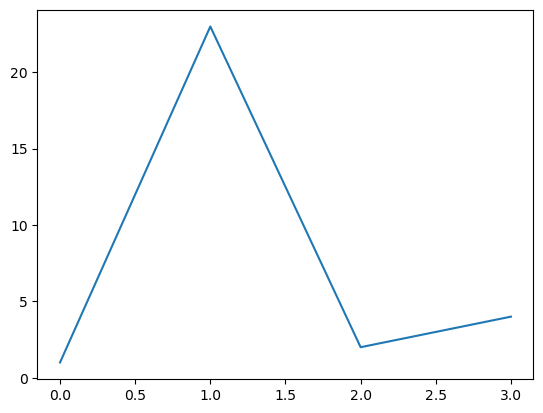
\includegraphics{Authoring_files/figure-pdf/fig-simple-output-1.png}

}

\caption{\label{fig-simple}Simple plot}

\end{figure}

\hypertarget{sec-equation}{%
\subsection{Equation}\label{sec-equation}}

\begin{equation}\protect\hypertarget{eq-stddev}{}{
std = \sqrt{\frac{1}{N-1} \sum_{i=1}^N(x_i - \overline{x})^2}
}\label{eq-stddev}\end{equation}

\begin{tcolorbox}[enhanced jigsaw, colframe=quarto-callout-note-color-frame, leftrule=.75mm, toptitle=1mm, arc=.35mm, opacitybacktitle=0.6, bottomrule=.15mm, breakable, colback=white, opacityback=0, coltitle=black, bottomtitle=1mm, rightrule=.15mm, titlerule=0mm, toprule=.15mm, title=\textcolor{quarto-callout-note-color}{\faInfo}\hspace{0.5em}{Note}, colbacktitle=quarto-callout-note-color!10!white, left=2mm]

test \texttt{note}

\end{tcolorbox}



\end{document}
